\documentclass{beamer}

\usetheme{Berlin}
\usecolortheme{crane}

% Custom yellow color scheme
\definecolor{UMYellow}{RGB}{255,193,7}
\definecolor{UMDarkYellow}{RGB}{245,166,35}
\definecolor{UMGold}{RGB}{255,179,0}

\setbeamercolor{structure}{fg=UMDarkYellow}
\setbeamercolor{palette primary}{bg=UMYellow,fg=black}
\setbeamercolor{palette secondary}{bg=UMDarkYellow,fg=white}
\setbeamercolor{palette tertiary}{bg=UMGold,fg=black}
\setbeamercolor{palette quaternary}{bg=UMDarkYellow,fg=white}
\setbeamercolor{titlelike}{parent=palette primary}
\setbeamercolor{block title}{bg=UMYellow,fg=black}
\setbeamercolor{block body}{bg=UMYellow!10,fg=black}
\setbeamercolor{frametitle}{bg=UMDarkYellow,fg=white}

% Remove navigation symbols and headline (progress bar)
\setbeamertemplate{navigation symbols}{}
\setbeamertemplate{headline}{}

\usepackage[utf8]{inputenc}
\usepackage[spanish]{babel}
\usepackage{graphicx}
\usepackage{amsmath}
\usepackage{hyperref}
\usepackage{subcaption}
\usepackage{booktabs}

\title{Visión Artificial}
\subtitle{BT3 y BT4}
\author[Gallego \& Vera]{Juan Diego Gallego Nicolás \\ Óscar Vera López}
\date{\today}
\institute{Universidad de Murcia}

\begin{document}

\frame{\titlepage}

\begin{frame}{Contenido}
  \tableofcontents
\end{frame}

\section{BT3: Hand-engineered features y reconocimiento robusto de objetos}

\begin{frame}{Comparación de Descriptores Locales}
  \begin{columns}
    \column{0.45\textwidth}
    \textbf{Métodos evaluados:}
    \begin{itemize}
      \item \textbf{AKAZE}: Más puntos, mejor repetibilidad
      \item \textbf{SIFT}: Robusto a escala, más lento
      \item \textbf{ORB}: Muy rápido, menos preciso
    \end{itemize}
    
    \textbf{Ratio test de Lowe} para filtrar matches incorrectos: 0.75

    \column{0.55\textwidth}
    \begin{figure}
      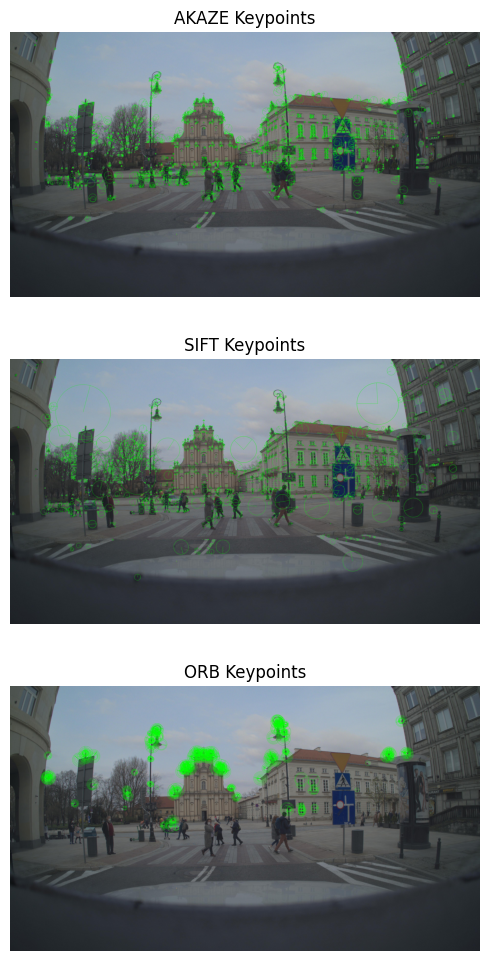
\includegraphics[width=0.56\textwidth]{images/keypoints_comparisons.png}
      \caption{Puntos clave detectados}
    \end{figure}
  \end{columns}
\end{frame}

\begin{frame}{Robustez ante Transformaciones}
  \begin{columns}
    \column{0.4\textwidth}
    \textbf{Repetibilidad por transformación:}
    
    \vspace{0.2cm}
    \textbf{Rotación:}
    \begin{itemize}
      \item AKAZE: 66.7\%
      \item SIFT: 61.8\%
      \item ORB: 63.0\%
    \end{itemize}
    
    \textbf{Escala:}
    \begin{itemize}
      \item SIFT: 43.4\% (mejor)
      \item AKAZE: 32.0\%
      \item ORB: 23.7\%
    \end{itemize}
    
    \column{0.6\textwidth}
    \begin{figure}
      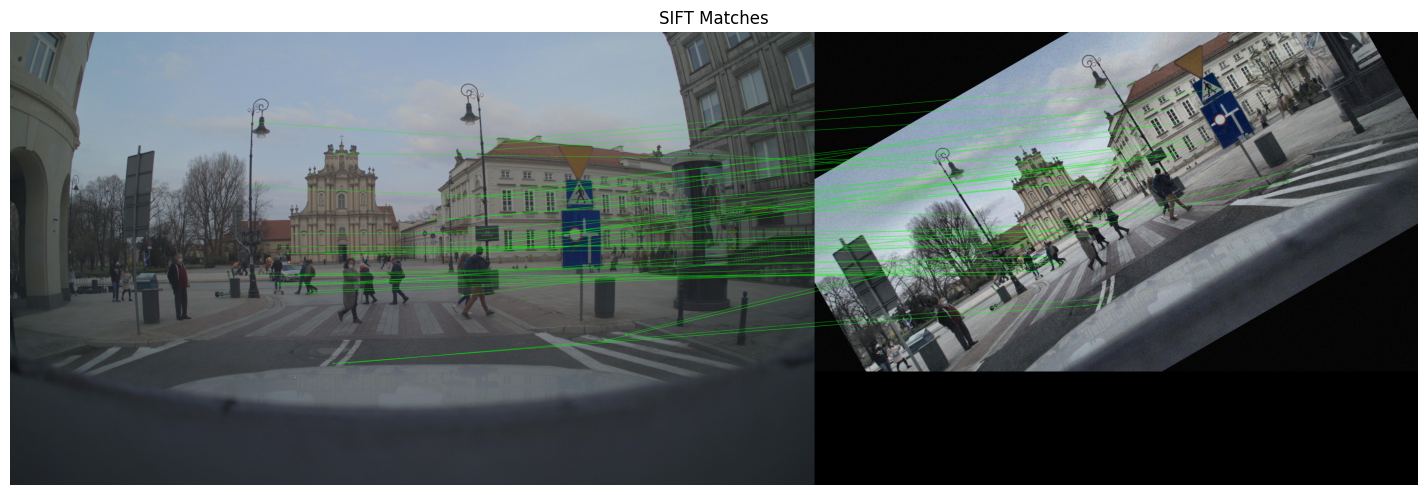
\includegraphics[width=\textwidth]{images/matching_sift_complex.png}
      \caption{Matching SIFT con transformación compleja}
    \end{figure}
  \end{columns}
\end{frame}

\begin{frame}{Template Matching con RANSAC}
  \begin{columns}
    \column{0.5\textwidth}
    \textbf{Proceso:}
    \begin{enumerate}
      \item Matching de descriptores
      \item Estimación homografía con RANSAC
      \item Localización de señales
    \end{enumerate}
    
    \vspace{0.3cm}
    \textbf{Limitaciones:}
    \begin{itemize}
      \item Variaciones de iluminación
      \item Templates sintéticos vs. reales
      \item Señales pequeñas = pocos keypoints
    \end{itemize}
    
    \column{0.5\textwidth}
    \begin{figure}
      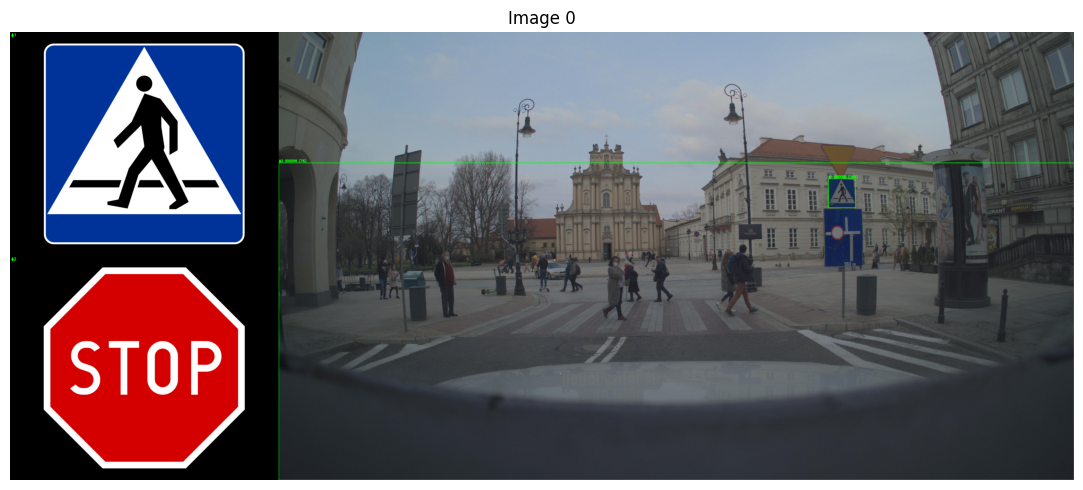
\includegraphics[width=\textwidth]{images/good_matching.png}
      \caption{Resultado de matching con RANSAC}
    \end{figure}
  \end{columns}
\end{frame}

\begin{frame}{Enfoque HOG+SVM}
  \textbf{Algoritmo HOG implementado desde cero:}
  \begin{enumerate}
    \item Cálculo de gradientes (Sobel)
    \item Histogramas por celda (8×8, 9 bins)
    \item Normalización L2-Hys por bloques (2×2)
    \item Vector de 1764 dimensiones
  \end{enumerate}
  
  \vspace{0.3cm}
  \textbf{Clasificación:}
  \begin{itemize}
    \item Ventana deslizante (64×64 px) a múltiples escalas
    \item SVM lineal entrenado con parches etiquetados
    \item 80\% train / 20\% test
  \end{itemize}
\end{frame}

\begin{frame}{Resultados: Clasificación de Parches}
  \begin{table}
    \centering
    \caption{Comparación de métricas F1-Score}
    \begin{tabular}{lccc}
      \toprule
      \textbf{Versión} & \textbf{Train} & \textbf{Test} \\
      \midrule
      skimage HOG & 0.712 & 0.816 \\
      Custom HOG & 0.799 & \textbf{0.850} \\
      Con preprocesado & 0.764 & 0.816 \\
      \bottomrule
    \end{tabular}
  \end{table}
  
  \vspace{0.3cm}
  \textbf{Observaciones:}
  \begin{itemize}
    \item Implementación custom supera a skimage (+3.4\%)
    \item Preprocesado HSV no mejora significativamente
    \item Precision en test muy alta ($>$90\%)
  \end{itemize}
\end{frame}

\begin{frame}{Resultados: Detección con Ventana Deslizante}
  \begin{table}
    \centering
    \footnotesize
    \begin{tabular}{lccc}
      \toprule
      \textbf{Métrica} & \textbf{skimage} & \textbf{Custom} & \textbf{Preproc.} \\
      \midrule
      Hit Rate & 92.0\% & \textbf{97.1\%} & 72.2\% \\
      GT Coverage & 10.9\% & 7.1\% & \textbf{12.4\%} \\
      F1-Score & 0.032 & 0.054 & 0.032 \\
      \bottomrule
    \end{tabular}
  \end{table}
  
  \vspace{0.3cm}
  \textbf{Análisis:}
  \begin{itemize}
    \item Alto Hit Rate: clasificación correcta por ventana
    \item Bajo GT Coverage: dificultad para cubrir señales reales
    \item Trade-off entre falsos positivos y cobertura
  \end{itemize}
\end{frame}

\begin{frame}{Comparación Visual de Detecciones}
  \begin{figure}
    \centering
    \begin{subfigure}[b]{0.32\textwidth}
      \centering
      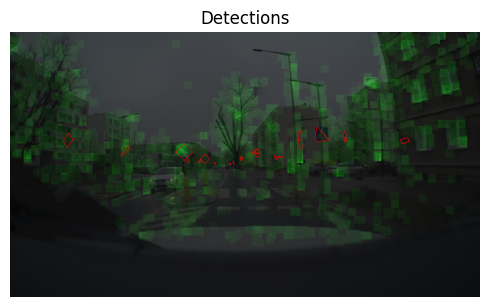
\includegraphics[width=\textwidth]{images/hog/skimage_5.png}
      \caption{skimage}
    \end{subfigure}
    \hfill
    \begin{subfigure}[b]{0.32\textwidth}
      \centering
      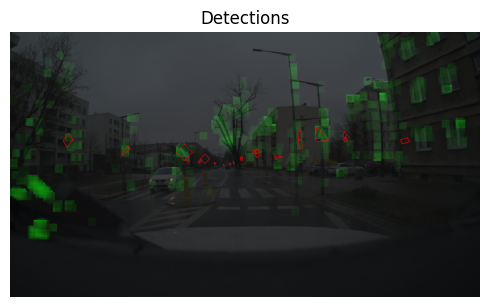
\includegraphics[width=\textwidth]{images/hog/custom_5.png}
      \caption{Custom}
    \end{subfigure}
    \hfill
    \begin{subfigure}[b]{0.32\textwidth}
      \centering
      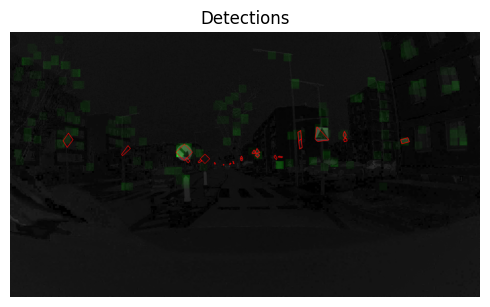
\includegraphics[width=\textwidth]{images/hog/pre_5.png}
      \caption{Preprocesado}
    \end{subfigure}
    \caption{Detección HOG+SVM en imagen de prueba}
  \end{figure}
\end{frame}

\section{BT4: Deep Learning para visión por computador}

\begin{frame}{YOLOv8 para Detección de Señales}
  
\begin{itemize}
  \item Arquitectura YOLOv8 nano y medium preentrenada en COCO
  \item Dataset de 2000 imágenes (80/20 split)
  \item Entrenamiento: 200 épocas con early stopping
  \item Métricas: mAP@0.5, mAP@0.5-0.95, precisión, recall
  \item Exportación a ONNX para inferencia rápida
\end{itemize}

\end{frame}

\begin{frame}{Resultados de entrenamiento}
  
\end{frame}

\end{document}
